\section{Korrelationsgrafer}
\label{DatabehandlingKorrelationsgrafer}
%
Når PCA analysen udføres relativt til højde, tyder det, som beskrevet i \fullref{DatabehandlingRHeight}, på, at en positiv korrelation mellem følgende parametre finder sted:
\begin{itemize}
	\item SQ12 og SQ18
	\item SQ14 og SQ15
	\item SQ8 og SQ17
\end{itemize}
%
Derudover ses der negativ korrelation mellem følgende parametre:
\begin{itemize}
	\item SQ12 og S21
	\item SQ18 og SQ21
	\item SQ2 og SQ9
	\item SQ4 og SQ9
	\item SQ16 og SQ19
\end{itemize}
%
For at undersøge dette nærmere opsættes relevante grafer, hvor forholdet mellem de forskellige parametre og skala spørgsmål visualiseres. På alle følgende grafer vil x-aksen indikere testpersoner, men ikke nødvendigvis i kronologisk rækkefølge, hvorfor værdier på x-aksen er fjernet.

På \autoref{fig:SammenligningSQ12SQ18} ses sammenhængen mellem SQ12 og SQ18, hvor der kan se en tendens i at når testpersonerne kan lide at blive betjent af robotten synes de også at robotten er spændende. 
%
\begin{figure}[H]
	\centering
	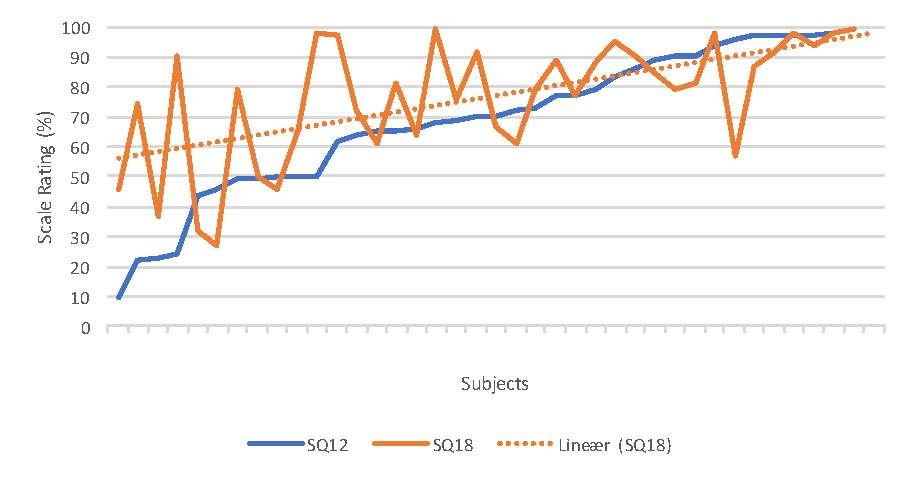
\includegraphics[width=\textwidth]{Figure/Korrelationsgrafer/SQ12+SQ18}
	\caption{Sammenhæng mellem hvad testpersonerne angiver (\%) på skalaen til SQ12: \textit{Jeg kan godt lide at blive betjent af robotten} og SQ18: \textit{Hvad synes du om robotten?}. At den orange kurve ikke er kontinuerlig skyldes, at nogle testpersoner ikke har angivet en respons på skalaen.}
	\label{fig:SammenligningSQ12SQ18}
\end{figure}
\noindent
%
På \autoref{fig:SammenligningSQ14SQ15} ses sammenhængen mellem SQ14 og SQ15. Kigges der på tendenslinjen kan der tilnærmelsesvis ses en sammenhæng mellem de to parametre, men kigges der på punkterne på grafen virker det ikke umiddelbart til at hvor personlig robottens hjælp blev oplevet og hvor overrasket testpersonerne blev over henvendelsen har indflydelse på hinanden.
%
\begin{figure}[H]
	\centering
	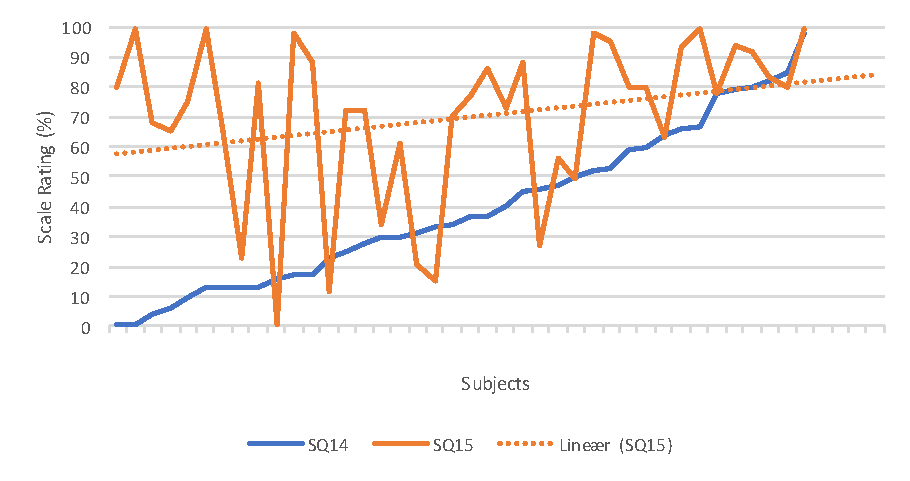
\includegraphics[width=\textwidth]{Figure/Korrelationsgrafer/SQ14+SQ15}
	\caption{Sammenhæng mellem hvad testpersonerne angiver (\%) på skalaen til SQ14: \textit{Hvor personlig oplevede du robottens hjælp?} og SQ15: \textit{Hvor overrasket blev du over robottens henvendelse?}.}
	\label{fig:SammenligningSQ14SQ15}
\end{figure}
\noindent
%
På \autoref{fig:SammenligningSQ8SQ17} ses der en lille tendens, hvor robotten rates mere elegant, når testpersonerne føler robotten kan hjælpe dem. Igen ligger datapunkterne dog meget spredt, så det betyder ikke nødvendigvis at en direkte sammenhæng er tilfældet. 
%
\begin{figure}[H]
	\centering
	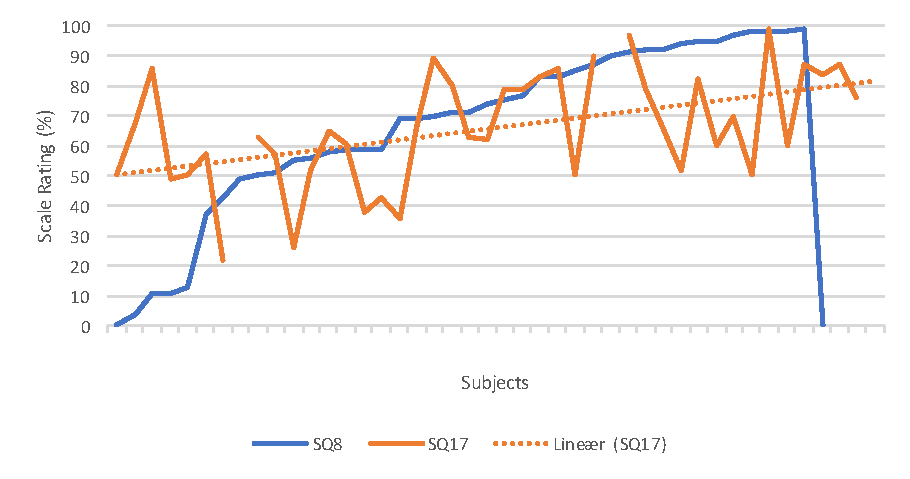
\includegraphics[width=\textwidth]{Figure/Korrelationsgrafer/SQ8+SQ17}
	\caption{Sammenhæng mellem hvad testpersonerne angiver (\%) på skalaen til SQ8: \textit{Jeg føler, at robotten kan hjælpe mig} og SQ17: \textit{Hvad synes du om robotten?}. At den orange kurve ikke er kontinuerlig skyldes, at nogle testpersoner ikke har angivet en respons på skalaen.}
	\label{fig:SammenligningSQ8SQ17}
\end{figure}
\noindent
%
På \autoref{fig:SammenligningSQ12SQ21} ses sammenhængen mellem SQ12 og SQ21, der har en negativ korrelation, jævnfør \autoref{fig:RHeight-Biplot}. Her ses det, at robotten anses som værende mindre anmasende, jo bedre testpersonerne kunne lide at blive betjent af robotten.
%
\begin{figure}[H]
	\centering
	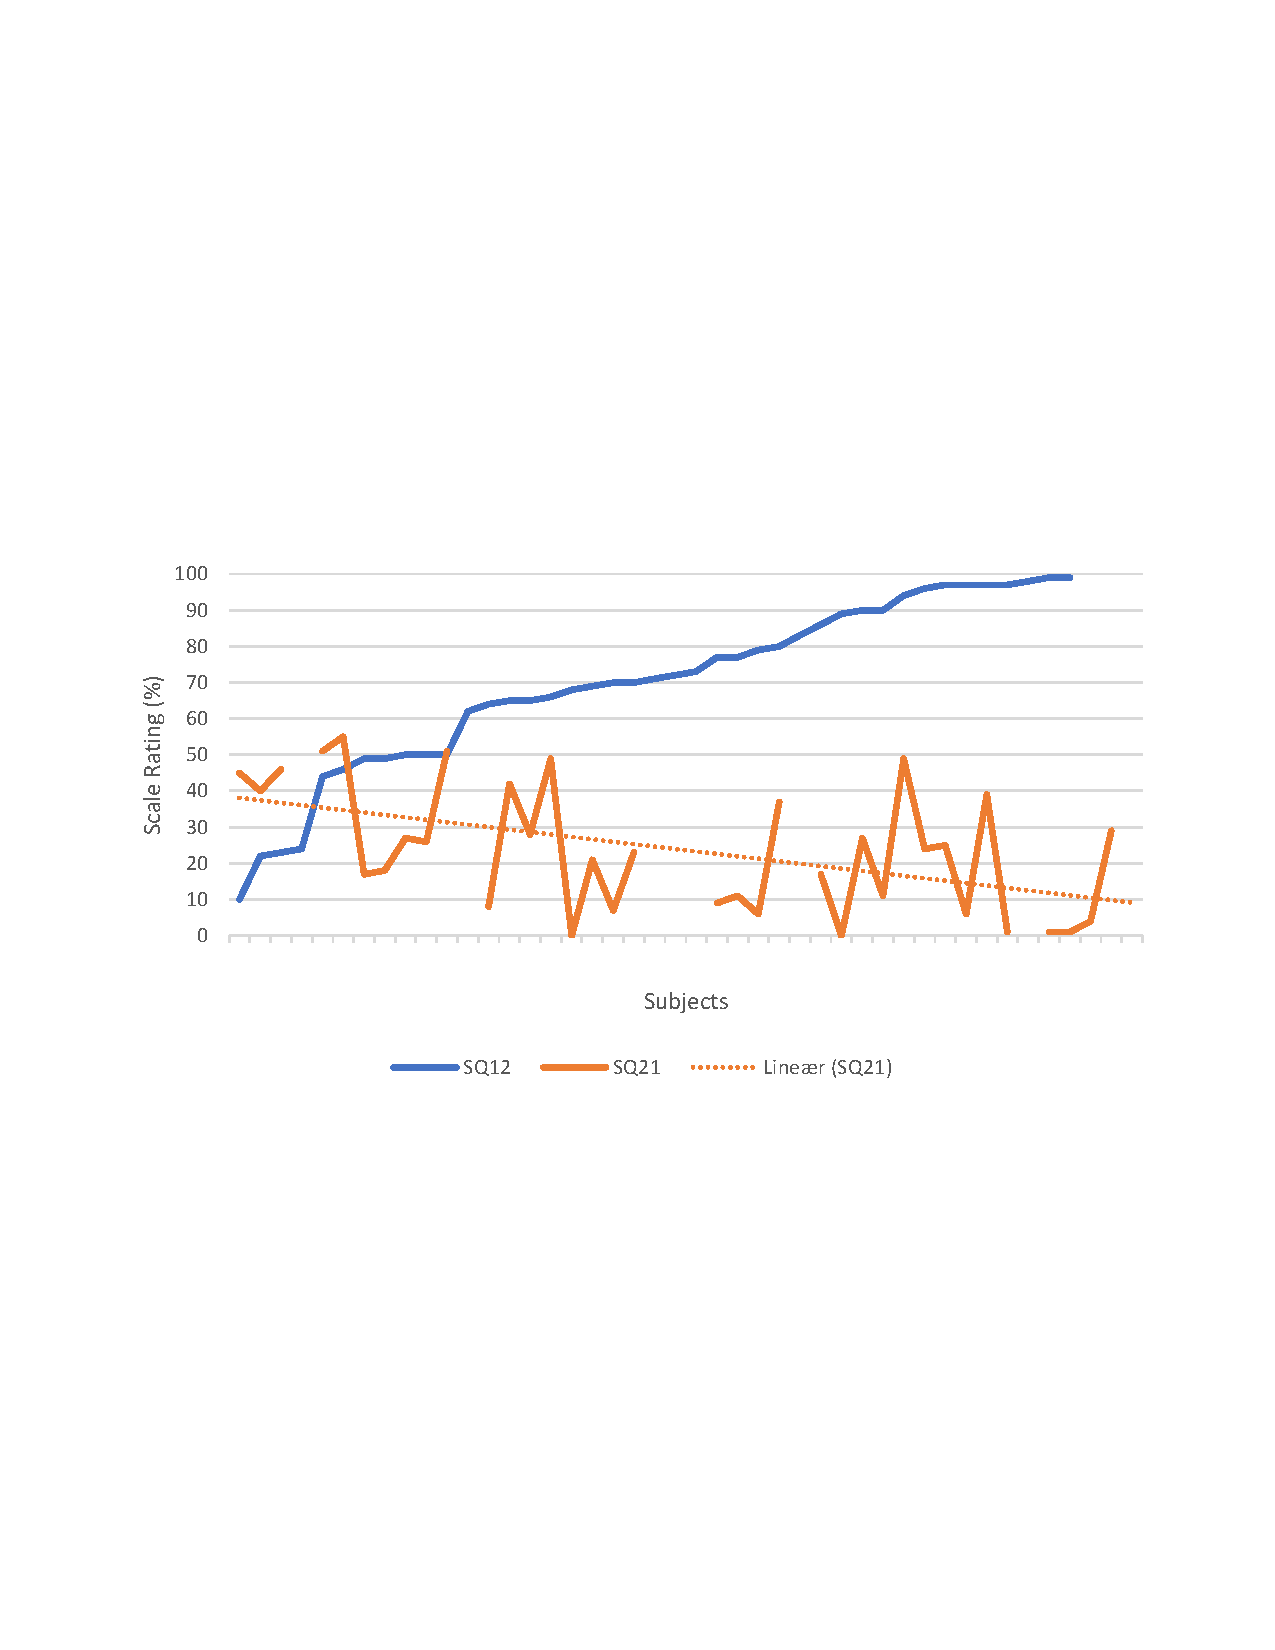
\includegraphics[width=\textwidth]{Figure/Korrelationsgrafer/SQ12+SQ21}
	\caption{Sammenhæng mellem hvad testpersonerne angiver (\%) på skalaen til SQ12: \textit{Jeg kan godt lide at blive betjent af robotten} og SQ21: \textit{Hvad synes du ellers om robotten?}. At den orange kurve ikke er kontinuerlig skyldes, at nogle testpersoner ikke har angivet en respons på skalaen.}
	\label{fig:SammenligningSQ12SQ21}
\end{figure}
\noindent
%
\autoref{fig:SammenligningSQ18SQ21} viser sammenhængen mellem SQ18 og SQ21. Her ses det, at det er en sammenhæng i testpersonernes ratings, da robotten anses som værende mindre anmasende, når robotten anses som værende mere spændende.
%
\begin{figure}[H]
	\centering
	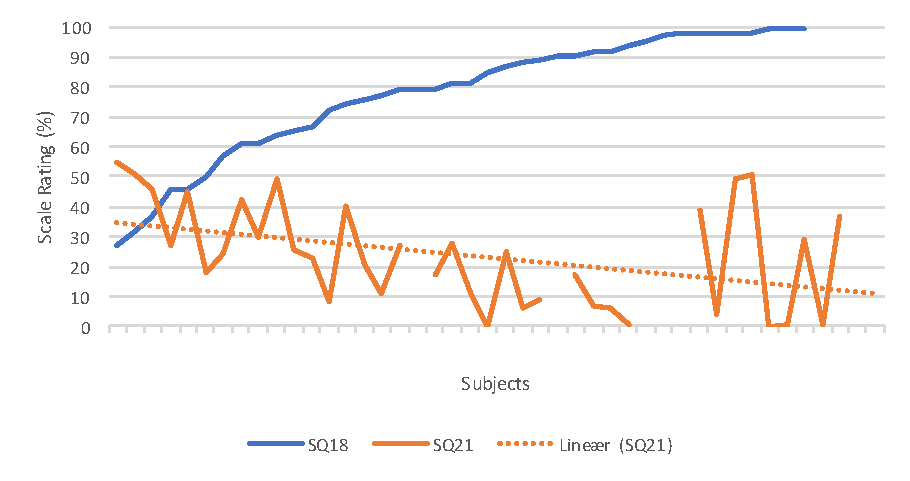
\includegraphics[width=\textwidth]{Figure/Korrelationsgrafer/SQ18+SQ21}
	\caption{Sammenhæng mellem hvad testpersonerne angiver (\%) på skalaen til SQ18: \textit{Hvad synes du om robotten} og SQ21: \textit{Hvad synes du ellers om robotten?}. At den orange kurve ikke er kontinuerlig skyldes, at nogle testpersoner ikke har angivet en respons på skalaen.}
	\label{fig:SammenligningSQ18SQ21}
\end{figure}
\noindent
%
På \autoref{fig:SammenligningSQ2SQ9} ses sammenhængen mellem SQ2 og SQ9. Figuren viser en lille tendens for, at ratings omkring hvorvidt robotten stod i vejen falder, når robotten opleves som mere imødekommende.
%
\begin{figure}[H]
	\centering
	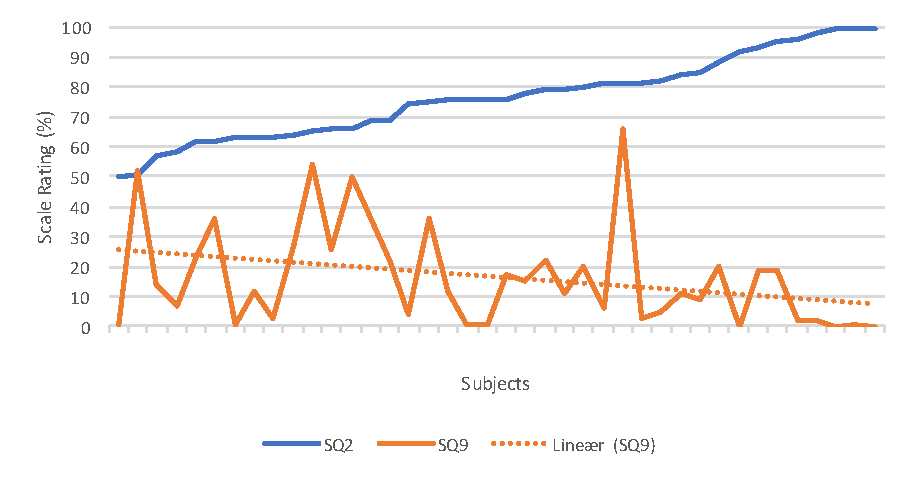
\includegraphics[width=\textwidth]{Figure/Korrelationsgrafer/SQ2+SQ9}
	\caption{Sammenhæng mellem hvad testpersonerne angiver (\%) på skalaen til SQ2: \textit{Hvordan oplevede du robotten?} og SQ9: \textit{Jeg synes, at robotten stod i vejen}. At den orange kurve ikke er kontinuerlig skyldes, at nogle testpersoner ikke har angivet en respons på skalaen.}
	\label{fig:SammenligningSQ2SQ9}
\end{figure}
\noindent
%
Selvom \autoref{fig:RHeight-Biplot} vise en negativ korrelation mellem SQ4 og SQ9, ses det på \autoref{fig:SammenligningSQ4SQ9}, at dette ikke nødvendigvis er tilfældet.
%
\begin{figure}[H]
	\centering
	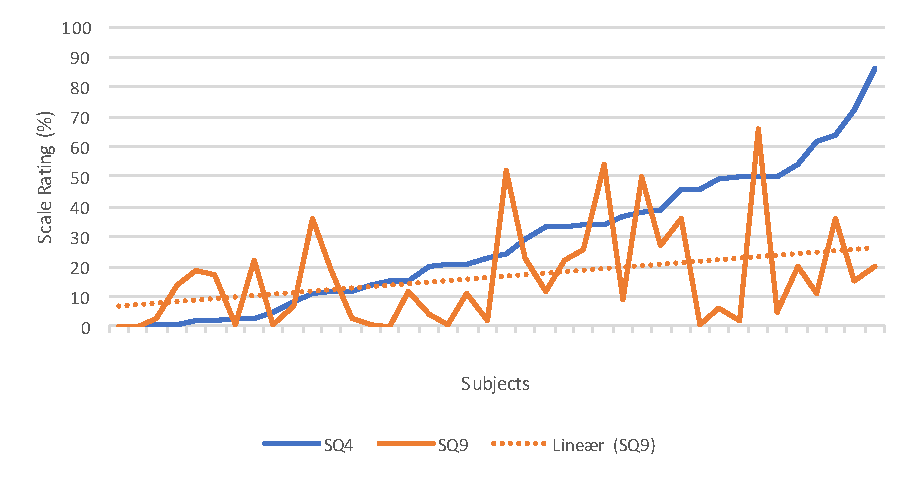
\includegraphics[width=\textwidth]{Figure/Korrelationsgrafer/SQ4+SQ9}
	\caption{Sammenhæng mellem hvad testpersonerne angiver (\%) på skalaen til SQ4: \textit{Hvordan oplevede du robottens bevægelser?} og SQ9: \textit{Jeg synes, at robotten stod i vejen}. At den orange kurve ikke er kontinuerlig skyldes, at nogle testpersoner ikke har angivet en respons på skalaen.}
	\label{fig:SammenligningSQ4SQ9}
\end{figure}
\noindent
%
\autoref{fig:SammenligningSQ16SQ19} ses sammenhængen mellem SQ16 og SQ19, hvor der ses en lille tendens af at testpersonerne synes robotten var mindre sød jo mere irriterende de synes den var. 
%
\begin{figure}[H]
	\centering
	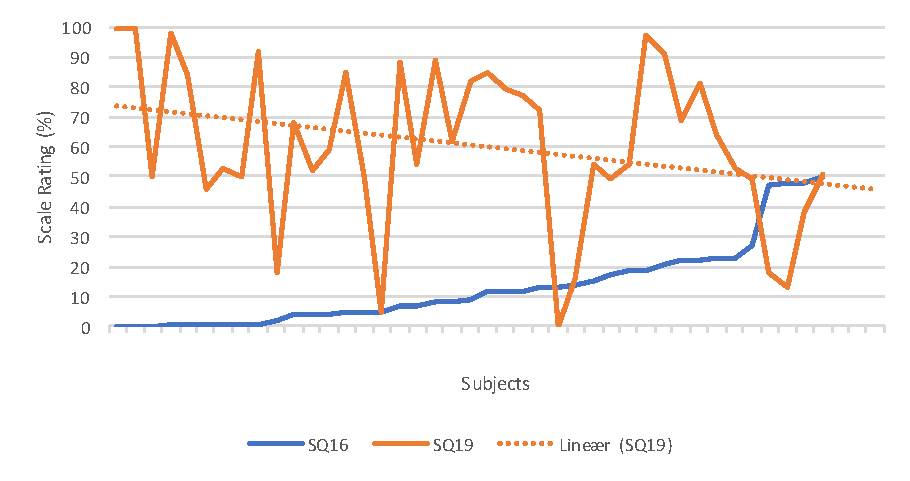
\includegraphics[width=\textwidth]{Figure/Korrelationsgrafer/SQ16+SQ19}
	\caption{Sammenhæng mellem hvad testpersonerne angiver (\%) på skalaen til SQ16 og SQ19, der begge har samme skala spørgsmål: \textit{Hvad synes du om robotten?} og forskellige labels.}
	\label{fig:SammenligningSQ16SQ19}
\end{figure}
\noindent
%
